\label{sec:cell-finite}
All ordinary labels are controllable. The interval requires exactly one workpiece, and new-start before old-stop is the only supplied precedence.
Table~\ref{tab:cell-finite-main} gives all component, endpoint-controller and monitor transitions, including the conventions for absent edges.
\begin{table}[!htbp]
\caption{Complete Cell components, controllers and monitors. $o/n$ denote old/new versions; $h/e$ mean holding/empty. Parentheses mark initial states. $m_A,m_B$ move to $A,B$; $j$ inspects at $B$.}
\label{tab:cell-finite-main}
\centering\small
\begin{tabular}{@{}>{\raggedright\arraybackslash}p{.16\linewidth}>{\raggedright\arraybackslash}p{.20\linewidth}p{.58\linewidth}@{}}\toprule
Object & States (initial) & Ordinary transitions\\\midrule
$A^o,A^n$ & $h,e$ ($h$) & $h\xrightarrow{m_B}e$, $e\xrightarrow{m_A}h$\\
$B^o$ & $h,e$ ($e$) & $e\xrightarrow{m_B}h$, $h\xrightarrow{m_A}e$\\
$B^n$ & $h,e$ ($e$) & $e\xrightarrow{m_B}h$, $h\xrightarrow{m_A}e$, $h\xrightarrow{j}h$\\
$C^o$ & $c_o$ ($c_o$) & $c_o\xrightarrow{m_A,m_B}c_o$\\
$C^n$ & $c_0,c_1$ ($c_0$) & $c_0\xrightarrow{m_A,j}c_0$, $c_0\xrightarrow{m_B}c_1$, $c_1\xrightarrow{j}c_0$, $c_1\xrightarrow{m_B}c_1$\\\midrule
$t_{r_{\rm one}}$ & $A,B,\mathsf{err}$ ($A$) & $A\xrightarrow{m_B}B$, $B\xrightarrow{m_A}A$, $A\xrightarrow{m_A}\mathsf{err}$, $B\xrightarrow{m_B}\mathsf{err}$\\
$t_{r_{\rm old}}$ & $k,\mathsf{err}$ ($k$) & $k\xrightarrow{j}\mathsf{err}$\\
$t_{r_{\rm inspect}}$ & $c,d,\mathsf{err}$ ($c$) & $c\xrightarrow{m_B}d$, $d\xrightarrow{j}c$, $d\xrightarrow{m_A}\mathsf{err}$\\\bottomrule
\end{tabular}
\par\smallskip\raggedright
$k,c,d$ mean old-safe, inspection-clear and inspection-pending; $c_0,c_1$ are distinct controller states.
Component/controller alphabets are exactly their displayed labels; unlisted edges are absent.
Unlisted non-error monitor edges self-loop, and $\mathsf{err}$ absorbs every label.
Each comma-separated label denotes an edge.\par
\end{table}


Endpoint tuples list stations $A,B$, controller and monitor. States $h/e$ mean holding/empty; $k,c,d$ mean old-safe, inspection-clear and inspection-pending; $c_o,c_0,c_1$ name controller states. Old reachable tuples are $x_A=(h,e,c_o,k)$ and $x_B=(e,h,c_o,k)$; new ones are $z_A=(h,e,c_0,c)$, $y_B=(e,h,c_1,d)$ and $z_B=(e,h,c_0,c)$. Initial tuples are $x_A,z_A$ and loadable targets are $\{z_A,z_B\}$, excluding pending inspection at $y_B$. The interval initializer records the holder at either all-old one-workpiece tuple. The new initializer admits all eight version-tagged one-workpiece tuples, installing $d$ when $B$ holds and $c$ otherwise. The paths starting with $A$/$B$ holding map to $z_B$/$z_A$ at handover.

With empty-only transfers $g_A=g_B=\{(e,e)\}$ and exactly one workpiece, the two paths $\rho_B;m_B;\mathsf{start};\mathsf{stop};j;\rho_A$ from $A$ holding and $\rho_A;m_A;\mathsf{start};\mathsf{stop};\rho_B$ from $B$ holding have safe singleton outcomes: start installs inspection-pending if $B$ holds and inspection-clear otherwise, stop removes the inspection ban, and both paths finish with new versions and clear inspection at matching supplied targets.
Their remaining lengths $6,\ldots,0$ and $5,\ldots,0$ strictly decrease, proving finite completion from both reachable old states (13 policy states and 11 edges).
Replacing the two transfer commands by one with relation $g_A\times g_B$, with endpoints and requirements fixed, requires both stations empty, but every ordinary move, inspection and requirement boundary preserves exactly one workpiece; that command can never execute, stays pending and makes every goal unreachable.

% Editorial prototype only. Exact states/actions/ranks from c24 figures/cell_paths.tex.
% Not included in c24, not a new experiment or proof.
\begin{figure}[!htbp]
\centering
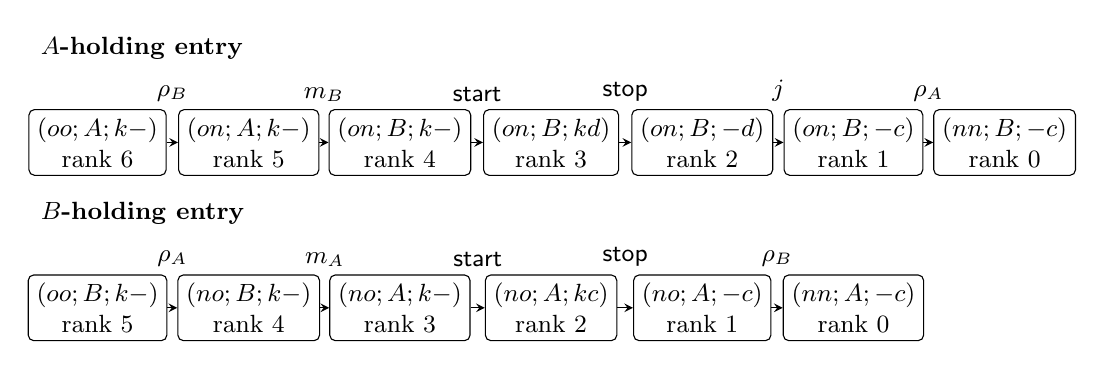
\begin{tikzpicture}[x=1.92cm,y=1cm,
  state/.style={draw,rounded corners=2pt,inner sep=3pt,font=\small,align=center},
  edge/.style={->,>=stealth},
  action/.style={font=\small,above,yshift=4mm}]
\node[anchor=west,font=\small\bfseries] at (-.44,1.2) {$A$-holding entry};
\node[state] (a0) at (0,0) {$(oo;A;k{-})$\\rank 6};
\node[state] (a1) at (1,0) {$(on;A;k{-})$\\rank 5};
\node[state] (a2) at (2,0) {$(on;B;k{-})$\\rank 4};
\node[state] (a3) at (3,0) {$(on;B;kd)$\\rank 3};
\node[state] (a4) at (4,0) {$(on;B;{-}d)$\\rank 2};
\node[state] (a5) at (5,0) {$(on;B;{-}c)$\\rank 1};
\node[state] (a6) at (6,0) {$(nn;B;{-}c)$\\rank 0};
\draw[edge] (a0)--node[action]{$\rho_B$}(a1);
\draw[edge] (a1)--node[action]{$m_B$}(a2);
\draw[edge] (a2)--node[action]{$\mathsf{start}$}(a3);
\draw[edge] (a3)--node[action]{$\mathsf{stop}$}(a4);
\draw[edge] (a4)--node[action]{$j$}(a5);
\draw[edge] (a5)--node[action]{$\rho_A$}(a6);
\node[anchor=west,font=\small\bfseries] at (-.44,-.9) {$B$-holding entry};
\node[state] (b0) at (0,-2.1) {$(oo;B;k{-})$\\rank 5};
\node[state] (b1) at (1,-2.1) {$(no;B;k{-})$\\rank 4};
\node[state] (b2) at (2,-2.1) {$(no;A;k{-})$\\rank 3};
\node[state] (b3) at (3,-2.1) {$(no;A;kc)$\\rank 2};
\node[state] (b4) at (4,-2.1) {$(no;A;{-}c)$\\rank 1};
\node[state] (b5) at (5,-2.1) {$(nn;A;{-}c)$\\rank 0};
\draw[edge] (b0)--node[action]{$\rho_A$}(b1);
\draw[edge] (b1)--node[action]{$m_A$}(b2);
\draw[edge] (b2)--node[action]{$\mathsf{start}$}(b3);
\draw[edge] (b3)--node[action]{$\mathsf{stop}$}(b4);
\draw[edge] (b4)--node[action]{$\rho_B$}(b5);
\end{tikzpicture}
\caption{One policy from both entries. States list versions of $A,B$, the workpiece holder, and old/new monitors; the holder also determines the interval monitor. A dash means inactive. Every edge decreases the remaining-step rank. The two rank-zero states match the respective fixed-controller targets.}
\label{fig:cell-paths}
\end{figure}

